\chapter{FUNDAMENTOS TEÓRICOS}


\section{BASE DE DATOS ESPACIO-TEMPORALES}

Dos campos que han surgido a mediados y finales de la década de 1980 son las  bases de datos espaciales y bases de
datos temporales las cuales se han convertido, en cierto modo como  las precursoras de las bases de datos
espacio-temporales.


\textbf{Base de datos espaciales} 

Las bases de datos espaciales tratan del eficiente almacenamiento y la recuperación de objetos en
el espacio que tienen identidad y extensión bien definidas, ubicaciones, así como ciertas relaciones geométricas
y / o topológica entre ellas, debido al desarrollo en campos de aplicación ( GIS, diseño VLSI, CAD) que necesita
tratar  con  grandes cantidades de entidades geométricas, geográficas o espaciales. Además de algunos estables y 
maduros prototipos basado en fundamentos algebraicos de tipo solido,   proveedores de sistemas gestores de bases de
datos comercial (DBMS) han ofrecido extensiones de sus productos, soportando tipos espaciales y operaciones
(Oracle Spatial, DB2 Spatial Extender, PostgresGIS , Microsoft SQL Server, MySQL). Sin lugar a dudas, los 
resultados en bases de datos espaciales han impulsado varias líneas de investigación importantes en bases
de datos de objetos en movimiento (MOD), como por ejemplo: consultas  populares de MOD (rango, 
vecino mas cercano),  propiedades topológicas y relaciones entre tipos espaciales. \cite{yuzheng2011}


\textbf{Base de datos temporales}


Muchas aplicaciones de bases de datos, como por ejemplo, contabilidad, gestión de cartera, registros médicos
y gestión de inventario; información que varia en el tiempo. El centro de las bases de datos temporales se
diferencia por:

\begin{description}
 \item [Tiempo válido de un hecho,] es el tiempo en el cual un dato particular es recogido y se convierte en verdad
 hasta donde el mundo representado por la base de datos es referida, 
posiblemente abarque el pasado, el presente y el futuro. Sin embargo, el tiempo válido no puede ser 
conocido, o los registros no pueden ser relevantes para las aplicaciones soportadas por la base de datos
o en el caso que los modelos de base de datos del  mundo real puedan variar entre los diferentes mundos reales.

\item [Tiempo de transacción de un hecho,] es el tiempo que un hecho dado es el actual en la base de datos. 
El tiempo de transacción puede asociarse con diferentes entidades de bases de datos, como, por ejemplo,
objetos y valores que no son hechos, porque no pueden ser verdaderos o falsos en forma aislada. Por lo tanto, todas las entidades de la base de datos tiene un aspecto de  tiempo de transacción, que tiene
una duración: desde inserción (lógico) a la eliminación de una determinada entidad.
\end{description}


Capturar el tiempo variable utilizando los modelos de datos tradicionales y lenguajes de consulta
puede ser una actividad engorrosa y, como consecuencia, se necesitan construcciones que permitirán
capturar los tiempos válidos y operación de los hechos, lo que conduce a relaciones temporales. Además,
en los lenguajes de consulta se necesitan  extensiones sintácticas que permiten las operaciones de base
de datos en modelos temporales.  \cite{yuzheng2011}

\section{TRAYECTORIAS}

Desde el punto de vista de los usuarios, el concepto de trayectoria se basa en la evolución de la posición de un 
objeto que se desplaza en el espacio durante un intervalo de tiempo dado. Por lo tanto, la trayectoria es por definición
un concepto espacio-temporal. Pero mientras este en movimiento puede ser visto como una característica de algunos de los
objetos que los diferencia de los objetos que no están en movimiento (por ejemplo, edificios, carreteras), el concepto que
un objeto se desplace implica que su movimiento está destinado a cumplir una meta significativa que requiere desplazarse
de un lugar a otro. Desplazarse para alcanzar un objetivo tiene una cantidad finita de tiempo (y cubre una cierta distancia
en el espacio), por lo tanto, las trayectorias son inherentemente definidas por un intervalo de tiempo. Este intervalo de
tiempo está delimitado por el instante en que el objeto comienza un desplazamiento (llamado $t_{inicio}$) y el instante en que
el recorrido termina ($t_{fin}$). Identificar $t_{inicio}$ y $t_{fin}$ dentro del  marco de tiempo del conjunto en que el objeto se mueve
es una decisión de la aplicación, es decir, una especificación basado en el usuario. La siguiente definición formal define
un punto de  trayectoria en movimiento en una perspectiva de base de datos.

\begin{description}
 \item [Definición 1 (Trayectoria)] Una trayectoria es el registro de usuario definido de la evolución de la posición
(pervivida como un punto) de un objeto que esta en movimiento en el espacio  durante un intervalo de tiempo dado con el fin de conseguir 
un objetivo dado.
  
  \begin{center}
  $[t_{inicio}$, $t_{fin}]$ $ \rightarrow $ Espacio
  \end{center}

\end{description}

La función del espacio de tiempo es definida por
el usuario y no es necesariamente el proporcionado por el mecanismo de adquisición de datos, cuya forma general es 
una secuencia de pares (punto de muestra, tiempo). Los datos sin procesar
a menudo tiene que someterse a un proceso de limpieza para corregir errores y aproximaciones en la adquisición de datos.
Además, la aplicación puede estar interesada en sólo un subconjunto de los puntos limpios de la muestra, por ejemplo,
omitiendo puntos adquiridos durante la noche y únicamente guardar movimiento en el día o sustitución de una secuencia
de puntos irrelevantes (desde la perspectiva de la aplicación) con un punto único representante 
(por ejemplo, para la representación de paradas como un punto único).

Otra diferencia importante entre un objeto con trayectorias y un objeto en movimiento  es que, para un 
objeto en movimiento, la función de espacio de tiempo 
que describe su posición se define sobre toda la vida útil del objeto. En su lugar, una trayectoria se da mediante
la restricción de la función a un intervalo de tiempo específico, $[t_{inicio}$,  $t_{fin}]$, 
incluido en el ciclo de vida del
objeto. Una trayectoria es un segmento de la ruta espacio-temporal cubierta por un objeto en movimiento 
(Figura~\ref{fig:ruta}). Por consiguiente, durante su vida útil de un objeto puede desplazarse un número de trayectorias,
una después de la otra. Por ejemplo, un pájaro tiene una trayectoria de migración en la primavera de 2006, desde
África a Europa, seguida de otra trayectoria en otoño de 2006 desde Europa a África, seguida de otras trayectorias 
en 2007, etc.

\begin{figure}
  \centering
  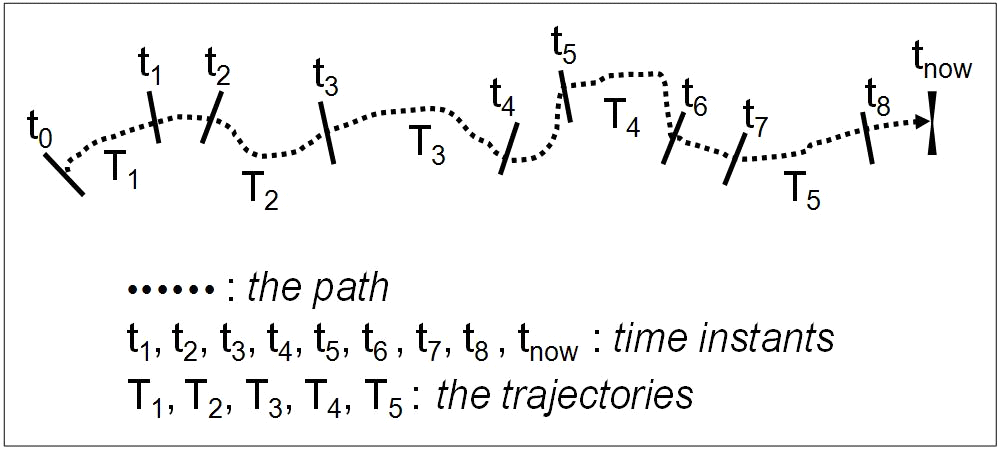
\includegraphics[scale=0.4]{pictures/trayectoria.png}
  \caption{Ruta Espacio Temporal \cite{spaccapietra2008conceptual}).}
  \label{fig:ruta}
\end{figure}

Para la Figura~\ref{fig:ruta}, una ruta espacio-temporal para un objeto en movimiento
en curso y sus muchas trayectorias definidas por una segmentación semántica de la ruta. En este ejemplo partes del
camino no pertenece a ninguna trayectoria, corresponden al movimiento que es irrelevante a la aplicación.
Los objetos que se desplazan no necesariamente se mueven continuamente durante una trayectoria. En consecuencia, las
trayectorias pueden ser ellas mismas segmentadas semánticamente mediante la definición de una secuencia temporal de
sub-intervalos de tiempo donde alternativamente la posición del objeto cambia y permanece fija. La primera se llama
movimiento y la segunda parada. Podemos ver entonces una trayectoria como una secuencia de movimientos que van de
una parada a la siguiente (o como una secuencia de paradas que separan los movimientos). Por ejemplo, un ave que se
ha apartado de la migración hará una parada en algún lugar durante algún tiempo para alimentarse, otra parada para
descansar, y así sucesivamente hasta que se alcanza el final de su trayectoria. Vendedores en viaje de negocios se
detendrán en todas las localidades donde planeaban encontrarse con un cliente.

Identificar paradas (y movimientos) dentro de una trayectoria es la responsabilidad de la aplicación. Paradas 
físicas (es decir, el hecho de que la posición del objeto es el mismo durante dos o más instantes consecutivos)
no se tienen en cuenta para las paradas conceptuales, ya que puede ser debido a eventos que son irrelevantes 
para la aplicación. Por ejemplo, la parada hecha por vendedor para beber un café es irrelevante para la
aplicación de seguimiento de la empresa. En su lugar, la parada de hecho para cumplir con 
un cliente es significativo. La aplicación podría estar interesado en contar el número 
de paradas por trayectoria, y, obviamente, las paradas que se cuentan son sólo las paradas
importantes. Se asume que se mueve y se para completamente para cubrir la trayectoria (es decir, 
no hay instante en [$t_{inicio}$, $t_{fin}$] que
no pertenezca ni a un movimiento ni a una parada).

Se definen semánticamente paradas y movimientos de la siguiente manera:

\begin{description}
 \item [Definición 2 (Parada)] Una parada es una parte de una trayectoria, de tal manera que:

El usuario ha definido explícitamente que es parte de la trayectoria ($[t_{inicioparadax}$, $t_{finparadax}]$) 
para representar una parada. La extensión temporal $[t_{inicioparadax}$, $t_{finparadax}]$ es un intervalo de tiempo
no vacía, y el objeto que se desplaza no se mueve (por lo que la vista de la aplicación de esta 
trayectoria se refiere), es decir, el rango espacial de la trayectoria para el intervalo 
$[t_{inicioparadax}$, $t_{finparadax}]$ es de un solo punto. Todas las paradas están temporalmente
disjuntas, es decir, la extensión temporal de dos paradas son siempre disjuntos.
\end{description}


\begin{description}
 \item [Definición 3 (Movimiento)] Un movimiento es una parte de una trayectoria, de tal manera que:

La parte está delimitada por dos extremidades que representan ya sea dos consecutivas paradas, o 
$t_{inicio}$ y la primera parada, o la última parada y $t_{fin}$, o $[t_{inicio}$, $t_{fin]}]$.

La extensión temporal $[t_{iniciomovimientox}$, $t_{finmovimientox}]$ es un intervalo de tiempo no vacía,y el 
rango espacial de la trayectoria para el intervalo $[t_{iniciomovimientox}$, $t_{finmovimientox}]$ es la línea 
espacio-temporal (no un punto) definido por la función de trayectoria (de hecho, es la línea poligonal 
construida sobre los puntos de muestreo en el intervalo $[t_{iniciomovimientox}$, $t_{finmovimientox}]$).
\end{description}


Desde el punto de vista de diseño de base de datos, un movimiento es un punto de tiempo variable 
definida en el intervalo de tiempo $[t_{iniciomovimientox}$, $t_{finmovimientox}]$. \cite{spaccapietra2008conceptual}

\section{IDENTIFICACIÓN DE PATRONES EN OBJETOS EN MOVIMIENTO}

Debido a la creciente disponibilidad de bases de datos espaciales, se han propuesto diferentes 
metodologías con el fin de encontrar información significativa que permanece oculta en este tipo de 
datos. Tratar de comprender cómo diversas entidades se mueven en un contexto espacial,  han 
demostrado ser útiles en temas tan diversos como el deporte \cite{iwase2004parallel}, la geografía 
socioeconómica \cite{frank2001life}, la migración de los animales \cite{dettki2004real} y la 
seguridad y la vigilancia \cite{makris2002path} \cite{piciarelli2006trajectory}. 

Los primeros enfoques de recuperación de información de bases de datos 
espacio-temporales incluyen para esto consultas destinadas a responder gama simple de predicado o 
consultas de vecinos más cercanos, por 
ejemplo, ``encontrar todos los objetos en movimiento dentro de la zona A entre las 10 a.m. a 
las 02:00 PM''  o "¿Cuántos coches condujeron entre la plaza principal y el aeropuerto el viernes". 
Extensiones de consultas espaciales en  paquetes comunes de software de SIG
y DBMS que son capaces de ejecutar este tipo de de consultas, sin embargo estas técnicas tratan de 
encontrar la mejor solución a explorar cada objeto espacial 
 a la vez de acuerdo con alguna métrica de distancia (por lo general euclidiana). Como 
resultados, es difícil de capturar el comportamiento colectivo y las correlaciones entre las 
entidades involucradas utilizando este tipo de consultas. 

Recientemente, han surgido unos nuevos intereses para la consulta de captura de patrones de ``grupo'' 
o conducta ``común'' entre las entidades en movimiento. De particular interés es el desarrollo 
de enfoques para identificar grupos de objetos en movimiento cuya participación en una relación 
fuerte y la interacción en una región espacial definida durante una duración de tiempo determinado. 
Algunos ejemplos de este tipo de enfoques son movimiento de cluster \cite{kalnis2005discovering} 
\cite{jensen2007continuous}, consultas de convoy \cite{jeung2008discovery-1} y patrones de 
agrupamiento \cite{gudmundsson2006computing} \cite{benkert2008reporting} \cite{VieiraT13} 
\cite{turdu2014}. 

Aunque diferentes interpretaciones pueden ser tomadas, un patrón de agrupamiento se refiere a un 
número predefinido de entidades que permanecen lo suficientemente cerca durante al menos un 
intervalo de tiempo dado. El desafiar a identificar este tipo de patrones de movimiento es 
especialmente relevante debido a la interacciones intrínsecas entre los miembros del grupo, 
especialmente en el contexto de los animales, peatones o vehículos. En esta investigación un marco 
alternativo para descubrir en movimiento  acuden patrones se propone. Esta investigación esta 
basada en un algoritmo existente denominado BFE propuesto por \cite{VieiraT13}, y otro 
llamado LCMFlock propuesto \cite{turdu2014} el cual extiende el algoritmo de BFE tomando ventaja de 
algoritmos de patrones frecuentes de minería en el area del aprendizaje de reglas de asociación.


\section{PATRÓN DE AGRUPAMIENTO}

\cite{vieira2009line} 
define patrones de agrupamiento también conocidos como flocks, como el problema de 
identificar todos los grupos 
de trayectorias que permanecen
``juntas'' por la duración de un intervalo de tiempo dado. Se Considera que los objetos en 
movimiento están suficientemente
cerca si existe un disco con un
radio dado que cubre todos los objetos que se mueven en el patrón 
(figura~\ref{fig:flockexample}). Una trayectoria satisface el 
patrón anterior, siempre y cuando suficientes trayectorias están contenidos 
dentro del disco para el intervalo de
tiempo especificado, es decir, la respuesta se basa no sólo en el comportamiento 
de una trayectoria dada, sino
también en las más cercanas a ella. Uno de los enfoques para descubrir patrones 
móviles de agrupamiento consiste
en encontrar un conjunto adecuado de discos en cada instante de tiempo y luego 
combinar los resultados de un 
instante de tiempo a otro. Como consecuencia, el rendimiento y el número de 
patrones encontrados depende del número
de los discos y cómo éstos se combinan.

En el ejemplo de la figura~\ref{fig:flockexample}, se muestra un patrón de 
agrupamiento el cual contiene tres 
trayectorias (T1, T2 y T3)
que están dentro de un disco en tres instantes de tiempo consecutivos. Los 
discos se pueden
mover libremente en el espacio bidimensional con el fin de acomodar los tres 
objetos en movimiento  y su centro no necesariamente
tiene que ser la localización de alguno de los objetos. Esto hace que el
descubrimiento de patrones sea mucho más complicada  porque hay un número 
infinito de posibles
colocaciones del disco en cualquier instante de tiempo y el posible número de 
combinaciones puede llegar a ser muy alta y costosa.

\begin{figure}
  \centering
  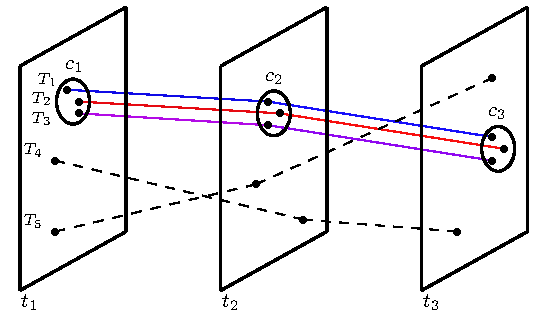
\includegraphics[scale=0.8]{pictures/flock_example.pdf}
  \caption{Ejemplo de patrones de agrupamiento \cite{vieira2009line}.}
  \label{fig:flockexample}
\end{figure}


\section{BFE (BASIC FLOCK EVALUATION)}

Este algoritmo en línea presentado por \cite{VieiraT13}, al parecer es el primer trabajo que 
presenta una solución exacta para reportar patrones de agrupamiento (flocks) en tiempo polinomial.

Un patron de agrupamiento Flock($\mu, \varepsilon, \delta$), esta definido de la siguiente manera:


\textbf{Definición:}  Dado un conjunto de trayectorias $\tau$ , un mínimo número de trayectorias 
$\mu >1 (\mu \in N)$, una máxima distancia $\epsilon > 0$ definida sobre la función de distancia d, 
y una duración de tiempo mínimo $\delta > 1 (\delta \in N)$. Un patron de agrupamiento
Flock($\mu, \epsilon, \delta$) reporta todas las colecciones máximas de tamaño F de 
trayectorias donde: para cada $f_{k}$ en F, el número de trayectorias en 
$f_{k}$ es mayor o igual que $\mu (|f_{k} | \geq \mu)$ y existen instancias de tiempo consecutivos 
$\delta$ 
tal que para cada $t_{i} \in [f_{k}^{t_{1}} ..f_{k}^{t_{1} + \delta} ]$,
hay un disco con centro $c_{k}^{t_{i}}$ y el radio $\epsilon / 2$ que cubre todo 
los puntos en $f_{k}^{t_{i}}$. Es decir: 
$\forall f_{k} \in F, \forall t_{i} \in [f_{k}^{t_{1}} ..f_{k}^{t_{1} + \delta}], \forall T_{j} \in 
f_{k}:  |f_{k}^{t_{i}}| \geq \mu, d(p_{j}^{t_{i}}, c_{k}^{t_{i}}) \leq \epsilon /2$

\section{PATRONES FRECUENTES EN BASE DE DATOS TRADICIONALES}

Patrones frecuentes son conjuntos de elementos, subsecuencias, o subestructuras que aparecen en un conjunto de datos con una
frecuencia no inferior a un umbral especificado por el usuario \cite{han2007frequent}. La cuestión de las modalidades 
interesantes desvelando en las bases de datos en diferentes contextos ha sido un tema de investigación
recurrente durante los últimos 15 años. Minería de datos general ha sido ampliamente reconocido como un
crítico campo por empresas de todo tipo. Como parte de los métodos de minería de datos, la tarea de aprendizaje 
de reglas de asociación han estudiado diferentes algoritmos de minería de patrones frecuente de identificar tendencias relevantes en los conjuntos de datos en diferentes disciplinas \cite{creighton2003mining} \cite{miller2009geographic} \cite{zhang2002association}. 

Una de las áreas en las que las técnicas de aprendizaje de reglas de asociación y el patrón frecuente 
algoritmos de minería se han aplicado con más frecuencia en el análisis de datos y tendencias del
mercado en transacciones de clientes de grandes supermercados y tiendas \cite{agrawal1994fast}. Por lo general, esta técnica 
tiene dado el nombre del problema de la cesta de compras a pesar de que los métodos derivados de resolverlo puede ser aplicado en diferentes contextos \cite{han2006data}.

El problema de la cesta de compras representa un intento por parte de un minorista para descubrir qué 
artículos de sus clientes compran con frecuencia juntos \cite{tsur1998query}. El objetivo es la comprensión de la 
comportamiento de un cliente típico y la identificación de los objetos de valor y relaciones 
entre ellos. Para este tipo de problema de la entrada es una base de datos con la información dada 
acerca de los artículos comprados. Cuando un cliente paga por sus productos en el cajero, un registro 
con los artículos comprados se inserta en la base de datos. En una vista general, es suficiente para 
capturar sólo el ID de la transacción y la identificación del producto (un registro por cada artículo comprado). 
Se le conoce como {TID: conjunto de elementos} esquema. Como los registros de la base de datos por lo general se refieren a 
transacciones, estas bases de datos se denominan bases de datos transaccionales. El objetivo de las compras 
análisis de la cesta es encontrar conjuntos de elementos (conjuntos de elementos) que están ``asociados'' y el hecho de 
su asociación a menudo se llama una regla de asociación \cite{tsur1998query}. 

Por ejemplo, si se sabe que un alto porcentaje de clientes están comprando leche y pan 
al mismo tiempo, en sus visitas a un supermercado, esta relación representa una regla de asociación. Se puede 
utilizar para formular nuevas estrategias de marketing, promociones, introducción de 
nuevos productos, diseño de catálogo, cruces de marketing o planificación de espacio en las
estanterías \cite{han2006data}. Es habitual localizar elementos asociados en diferentes pasillos y de alta rentabilidad
o nuevos productos entre ellos para asegurarse de que están expuestos a más clientes \cite{tsur1998query}. \cite{giudici2005applied} analizan 
otros casos de estudio aplicados en el comercio y el marketing, donde se exploran métodos diferentes reglas
de asociación. durante los últimos años muchas mejoras y nuevas técnicas se han desarrollado y propuesto 
con el fin de mejorar y tomar ventaja de los beneficios del análisis de reglas de asociación.

\section{LCM (LINEAR TIME CLOSED ITEMSET MINER)}

El problema de LCM propuesto por \cite{uno2005lcm} se define de la siguiente manera.

Sea I un conjunto de elementos. Sea D una base de datos transaccional de tal manera que cada 
registro (llamada transacción) es un conjunto de elementos. La frecuencia de un conjunto de 
elementos es el número de transacciones, incluyendo el conjunto de elementos. Para un número dado t 
(llamado soporte), un conjunto de elementos se dice que es frecuente si su frecuencia es no menos de 
t. Un conjunto de elementos frecuente se llama máxima si está incluido en ningún otro conjunto de 
elementos frecuentes, y se llama cerrada si está incluido en ningún otro conjunto de elementos de la 
misma frecuencia. La tarea de LCM, es enumerar (sacar, o contar) todos los conjuntos de elementos 
frecuentes, todos los conjuntos de elementos frecuentes máximos, o todos los conjuntos de elementos 
frecuentes cerrados en una base de datos transaccional para un soporte dado.